\documentclass[tikz,border=5pt]{standalone}
\usepackage{tikz}
\usetikzlibrary{arrows.meta,positioning}
\begin{document}
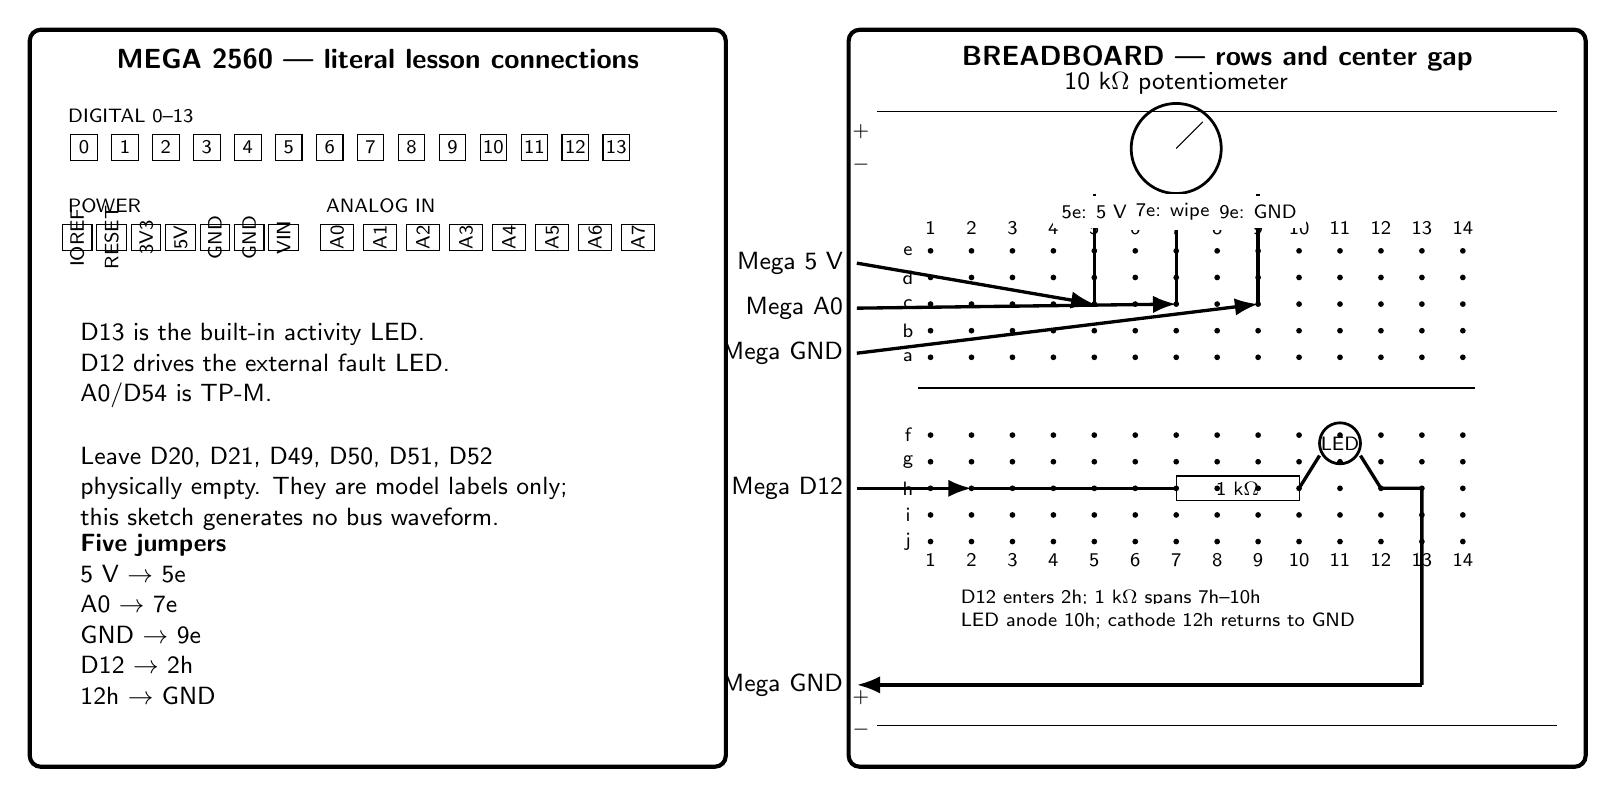
\begin{tikzpicture}[x=0.52cm,y=0.52cm,>=Latex,
  wire/.style={line width=1.2pt}, note/.style={font=\sffamily\small},
  tiny/.style={font=\sffamily\scriptsize}]
  \draw[line width=1.5pt,rounded corners] (0,0) rectangle (17,18);
  \node[note,font=\sffamily\bfseries] at (8.5,17.3) {MEGA 2560 --- literal lesson connections};
  \node[tiny,anchor=west] at (0.7,15.9) {DIGITAL 0--13};
  \foreach \x/\n in {1/0,2/1,3/2,4/3,5/4,6/5,7/6,8/7,9/8,10/9,11/10,12/11,13/12,14/13}
    {\draw (\x,14.8) rectangle ++(0.65,0.65); \node[tiny] at (\x+0.325,15.125) {\n};}
  \node[tiny,anchor=west] at (0.7,13.7) {POWER};
  \foreach \x/\n in {0/IOREF,1/RESET,2/3V3,3/5V,4/GND,5/GND,6/VIN}
    {\draw (0.8+\x*0.84,12.6) rectangle ++(0.72,0.65);
     \node[tiny,rotate=90] at (1.16+\x*0.84,12.925) {\n};}
  \node[tiny,anchor=west] at (7.0,13.7) {ANALOG IN};
  \foreach \x/\n in {0/A0,1/A1,2/A2,3/A3,4/A4,5/A5,6/A6,7/A7}
    {\draw (7.1+\x*1.05,12.6) rectangle ++(0.8,0.65);
     \node[tiny,rotate=90] at (7.5+\x*1.05,12.925) {\n};}
  \node[note,align=left,anchor=west] at (1,9.8)
    {D13 is the built-in activity LED.\\D12 drives the external fault LED.\\A0/D54 is TP-M.};
  \node[note,align=left,anchor=west] at (1,6.8)
    {Leave D20, D21, D49, D50, D51, D52\\physically empty. They are model labels only;\\this sketch generates no bus waveform.};

  \draw[line width=1.5pt,rounded corners] (20,0) rectangle (38,18);
  \node[note,font=\sffamily\bfseries] at (29,17.3) {BREADBOARD --- rows and center gap};
  \foreach \x in {1,...,14} {
    \foreach \y in {0,...,4} {\fill (21+\x,10+\y*0.65) circle (0.07);}
    \foreach \y in {0,...,4} {\fill (21+\x,5.5+\y*0.65) circle (0.07);}
    \node[tiny] at (21+\x,13.15) {\x};
    \node[tiny] at (21+\x,5.05) {\x};
  }
  \foreach \y/\n in {0/a,1/b,2/c,3/d,4/e}
    {\node[tiny] at (21.45,10+\y*0.65) {\n};}
  \foreach \y/\n in {0/j,1/i,2/h,3/g,4/f}
    {\node[tiny] at (21.45,5.5+\y*0.65) {\n};}
  \draw (21.7,9.25)--(35.3,9.25);
  \draw (20.7,16)--(37.3,16);
  \draw (20.7,1)--(37.3,1);
  \node[tiny] at (20.3,15.5) {$+$}; \node[tiny] at (20.3,14.7) {$-$};
  \node[tiny] at (20.3,1.7) {$+$}; \node[tiny] at (20.3,0.9) {$-$};

  % potentiometer, three distinct legs
  \draw[line width=1pt] (28,15.1) circle (1.1);
  \draw (28,15.1)--(28.65,15.75);
  \draw[wire] (26,14)--(26,11.3);
  \draw[wire] (28,14)--(28,11.3);
  \draw[wire] (30,14)--(30,11.3);
  \node[note] at (28,16.7) {10 k$\Omega$ potentiometer};
  \node[tiny,fill=white] at (26,13.55) {5e: 5 V};
  \node[tiny,fill=white] at (28,13.55) {7e: wiper};
  \node[tiny,fill=white] at (30,13.55) {9e: GND};

  % fault branch
  \draw[wire] (23,6.8)--(28,6.8);
  \draw (28,6.5) rectangle (31,7.1);
  \node[tiny] at (29.5,6.8) {1 k$\Omega$};
  \draw[wire] (31,6.8)--(31.5,7.6);
  \draw[line width=1pt] (32,7.9) circle (0.5);
  \draw[wire] (32.5,7.6)--(33,6.8)--(34,6.8)--(34,2);
  \node[tiny,anchor=west,fill=white] at (22.5,4.1)
    {D12 enters 2h; 1 k$\Omega$ spans 7h--10h};
  \node[tiny,anchor=west,fill=white] at (22.5,3.55)
    {LED anode 10h; cathode 12h returns to GND};
  \node[tiny] at (32,7.9) {LED};

  % short, non-crossing net callouts; the nearby hole names are authoritative
  \draw[wire,->] (20.2,12.3)--(26,11.3);
  \node[note,anchor=east] at (20.1,12.3) {Mega 5 V};
  \draw[wire,->] (20.2,11.2)--(28,11.3);
  \node[note,anchor=east] at (20.1,11.2) {Mega A0};
  \draw[wire,->] (20.2,10.1)--(30,11.3);
  \node[note,anchor=east] at (20.1,10.1) {Mega GND};
  \draw[wire,->] (20.2,6.8)--(23,6.8);
  \node[note,anchor=east] at (20.1,6.8) {Mega D12};
  \draw[wire,<-] (20.2,2)--(34,2);
  \node[note,anchor=east] at (20.1,2) {Mega GND};

  \node[note,align=left,anchor=west] at (1,3.6)
    {\textbf{Five jumpers}\\5 V $\rightarrow$ 5e\\A0 $\rightarrow$ 7e\\
     GND $\rightarrow$ 9e\\D12 $\rightarrow$ 2h\\12h $\rightarrow$ GND};

\end{tikzpicture}
\end{document}
